%%%%%%%%%%%%%%%%%%%%%%%%%%%%%%%%%%%%%%%%%%%%%%%%%%%%%%%%%%%%%%%%%%
%%        mmm  mmmmmm mm   m        m    m mmmmmm  mmmm         %%
%%      m"   " #      #"m  #        #    # #      "   "#        %%
%%      #   mm #mmmmm # #m #        #    # #mmmmm   mmm"        %%
%%      #    # #      #  # #  """   #    # #          "#        %%
%%       "mmm" #mmmmm #   ##        "mmmm" #mmmmm "mmm#"        %%
%%                                                              %%
%%                                                              %%
%%                                                              %%
%%      Grundlagen der Elektrischen Netzwerke, UE               %%
%%      Gruppe 5, Team F                                        %%
%%      Authors: Severin Wolf, Maximilian Seidler.              %%
%%%%%%%%%%%%%%%%%%%%%%%%%%%%%%%%%%%%%%%%%%%%%%%%%%%%%%%%%%%%%%%%%%
\documentclass[a4paper]{article}
\usepackage{amsmath}
\usepackage[utf8]{inputenc}
\usepackage[T1]{fontenc}
\usepackage[english]{babel}
\usepackage{geometry}
\usepackage{graphicx}
\usepackage{tikz}
\usepackage{listings}
\geometry{a4paper,left=3cm,right=2cm, top=2cm, bottom=2cm} 
\usepackage[EFvoltages, european, straightvoltages]{circuitikz}

%tikz
\ctikzset{resistor = european}
\usetikzlibrary{decorations.pathreplacing}

%no paragraph indent
\setlength{\parindent}{0pt}

%for math, that does not fit
\renewcommand*{\arraystretch}{1.3}
\newcommand\scalemath[2]{\scalebox{#1}{\mbox{\ensuremath{\displaystyle #2}}}}

\newcommand\blfootnote[1]{%
	\begingroup
	\renewcommand\thefootnote{}\footnote{#1}%
	\addtocounter{footnote}{-1}%
	\endgroup
}

% upright differenzial symbol with good spacing included!!!
\makeatletter
\providecommand*{\diff}%
	{\@ifnextchar^{\DIfF}{\DIfF^{}}}
\def\DIfF^#1{%
	\mathop{\mathrm{\mathstrut d}}%
		\nolimits^{#1}\gobblespace
}
\def\gobblespace{%
	\futurelet\diffarg\opspace}
\def\opspace{%
	\let\DiffSpace\!%
	\ifx\diffarg(%
		\let\DiffSpace\relax
	\else
		\ifx\diffarg\[%
			\let\DiffSpace\relax
		\else
			\ifx\diffarg\{%
				\let\DiffSpace\relax
			\fi\fi\fi\DiffSpace}

\begin{document}
\pagestyle{empty} \enlargethispage*{25cm}\samepage{
\vspace*{-3cm}
\begin{center}
\begin{minipage}[!h]{16cm}
\hspace*{0.2cm}

\includegraphics[width=3.3cm]{./Figures/igte_logo}
\begin{tabular}{p{8cm}}
\vspace{0.2cm}
\centering{
\Large Institute of Fundamentals and Theory in
 Electrical Engineering\\
Graz University of Technology\\
~\\}
\end{tabular}

\includegraphics[width=3.3cm]{./Figures/TUG_logo}
\end{minipage}
		\Large
		\textbf{Fundamentals of electrical circuits} \vspace*{0.5cm}\\
		\textbf{2. Homework}\\Th$\acute{\text{e}}$venin Equivalent Circuit and Linearity
		\vspace*{0.5cm}
		
		\large
		18 March 2021
	\end{center}}
	
	\vspace*{1cm}
	
	%%%%%%%%%%%%%%%%%%%%%%%%%%%%%%%%%%%%%%%%%%%%%%%%%%%%%%%%%%%%%%%%%%%%
	%%%%%%%%%%%%%%%%%%%%%%%%%%%%%%%%%%%%%%%%%%%%%%%%%%%%%%%%%%%%%%%%%%%%
	\section*{Assignment 1}
	Consider the depicted circuit in figure \ref{fig:circuit_hw3}. The switch has been in position \textbf{a} for a long time and changes to position \textbf{b} instantaneously at $t=T_0$.

	\begin{enumerate}
		
		\item The expression for the continuous quantity x(t) as a function of time at the
                   inductance L for $t \geq T_0$ \textbf{after} the switch changed its position from a to b should be determined. 
		
		\begin{itemize}
			\item Determine the initial value $x_0$ for the contiuous quantity at the inductance $L$ \textbf{before} the switch changed from position a to b. There are different approaches. Either apply Kirchhoff's laws and explicitly depict the value of interest, the node voltage method (write down equations \textbf{or} determine the matrix by ovserving the circuit and solve it with MatLab) or use the principle of superposition (calculate the effect of every source individually on the value of interest and sum the effects up with respect to the correct sign). 
			\item Apply Kirchhoff's current law (KCL) and Kirchhoff's voltage law (KVL)  for the case $t \geq T_0$ to derive the required mesh and node eqations for the given circuit.
			\item Derive the first order differential equation for the continuous quantity x(t). \\
				  \textbf{hint:} $x' + A x = B$.
			\item Determine the homogeneous solution by applying the Ansatz $x_h = K \cdot e^{-\lambda (t - T_0)}$.
			\item Determine the particular solution by applying the Ansatz $x_p = A$ (constant).
			\item Solve the initial value problem (determine K) by using the previously calculated initial condition $x_0$ at $t=T_0$ for the continuous quantity x(t).
		\end{itemize}
	
		\item Use the general solution for transient response $\mathbf{x(t) = x_f + [x_0 - x_f ] \cdot e^{-\frac{t-t_0}{\tau}}}$ and compare both results.
		
		\item Simulate the given problem in LTspice over the time period $0\,s \leq t \leq 5\tau + T_0$ in order to confirm your calculated results. Plot the voltage across the inductor $u_L(t)$ and the current $i_L(t)$. Compare the results with your calculations and discuss the findings with a few words.\\
		      \textbf{hint:} The changing of the switch from position \textbf{a} to \textbf{b} can be realized by replacing it with two voltage controlled switches and pulsed voltage source. One of the switches opens and one of them closes simultaneously at $t=T_0$. Use the switch from \textbf{switch\_example.asc}
		
	\end{enumerate}

	\subsection*{given values:}
	$R_1 = 2\,\Omega$ \qquad $R_2 = 4\,\Omega$ \qquad $R_3 = 3\,\Omega$ \qquad $R_4 = 2\,\Omega$ \qquad $R_5 = 3\,\Omega$ \qquad $R_6 = 5\,\Omega$ \\
	$L = 5\, mH$  \qquad $U_{s1} = 4\,V$ \qquad  $I_{s2} = 300\,mA$ \qquad $U_{s3} = 1\,V$
        \qquad $T_0 = 1~ms$
	
	\blfootnote{Deadline: 15th April 2021; \qquad presentation: Group no. 3}
	
	\newpage
%	\begin{figure}[h!]
%		\centering
%		\includegraphics[scale=0.75]{./Figures/homework3_circuit.eps}
%		\caption{Given circuit for assignment 3}
%		\label{fig:circuit_hw3}
%	\end{figure}

\begin{figure}[h!] \centering    
   \begin{circuitikz}[scale=0.75, transform shape]
      %Switch
      \node[spdt, rotate=90] (SW) at (5,5.4)              {};
      %Us_1
      \draw (0,0) to[V, v_=$U_{S1}$, color=blue]        (0,6);
      %Us_2
      \draw (10,6) to[V, v=$U_{S3}$, color=blue]        (10,0);
      %Is_2
      \draw (0,8) to[I, i=$I_{S2}$, color =red]         (-5,8);
      %R_1
      \draw (0,0) to[R, -*, l=$R_1$]                    (5,0);
      %R_2
      \draw (-5,6) to[R, -*, l=$R_2$]                   (0,6);
      %R_3
      \draw (0,6) to[R, -*, l=$R_3$]                    (4,6)
      to[short] (SW.out 1);
      %R_4
      \draw (SW.in) to[R, l=$R_4$, i=$i_{l}$]           (5,2.5);
      %R_5
      \draw (SW.out 2) to[R, -*, l=$R_5$]               (8,6);
      %R_6
      \draw (8,6) to[R, *-*, l=$R_6$]                   (8,0);
      %L
      \draw (5,2.5) to[L, l=$L$, v=$u_{L}$]             (5,0);
      %connections
      \draw (-5,8) to[short] (-5,6);
      \draw (5,0) to[short] (10,0);
      \draw (8,6) to[short] (10,6);
      \draw (0,8) to[short] (4,8) to[short] (4,6);
      %clamps + connections
      %\draw (7.5,6) to[short, o-] (11,6);
      %\draw (7.5,3) to[short, o-] (11,3);
      %nodes
      \node[above]               (a) at (SW.out 1) {$(a)$};
      \node[above]               (b) at (SW.out 2) {$(b)$};
      %\node[above]              (n_1) at (3,6) {$n_1$};
      %\node[above, xshift=3mm]  (n_3) at (3,3) {$n_2$};
      %\node[above, xshift=3mm]  (n_4) at (6,3) {$n_3$};
      %\node[below]              (ref) at (3,0) {ref};
      %\node[above]              (a) at (7.5,6) {a};
      %\node[above]              (b) at (7.5,3) {b};
\end{circuitikz}
\caption{Given circuit for assignment 3}
\label{fig:circuit_hw3}
\end{figure}


\tableofcontents
\listoffigures
\clearpage

\section{Solution}
\subsection{Analytical calculations}
\subsubsection{Initial value $x_{0}$}
When the switch in figure (\ref{fig:circuit_hw3}) is set to be at $(a)$ for a long time, we can
simplify the circuit to be to following. \\
\begin{figure}[h!] \centering    
\begin{circuitikz}
      %Us_1
      \draw (0,0) to[V, v_=$U_{S1}$, color=blue]        (0,2.5);
      %Is_2
      \draw (0,5) to[I, i=$I_{S2}$, color =red]         (5,5);
      %R_1
      \draw (0,0) to[R, l=$R_1$]                        (5,0);
      %R_2
      \draw (0,2.5) to[R, l=$R_2$]                      (0,5);
      %R_3
      \draw (0,2.5) to[R, *-*, l=$R_3$]                 (5,2.5);
      %R_4
      \draw (5,2.5) to[R, l=$R_4$, i=$i_{l}$]           (5,0);
      %connections
      \draw (5,5)   to[short]                           (5,2.5);
\end{circuitikz} 
\caption{circuit state at $T_0$}
\label{fig:circuit_a}
\end{figure}
\\ In an ideal world the Inductor $L$ has become a short. In reality, the equivalent series
resistance is very small $<<1\Omega$. Our disired current value for $x_{0}$, which is $i_{L}$ at
$T_{0}=1ms$ will be calculated using the principle of superposition. 
\subsubsection*{$U_{S1}$ is active, $I_{S2}$ is off.} 
The powersupply $I_{S2}$ acts as a open circuit, so there is also no current flowing throught
$R_2$. The current $i_{L}$ is now the same across every resistor in the circuit. We will calculate
its value with $i_{L}(T_0)' = \frac{U_{S1}}{R_{ges}}$.
 \[
   R_{ges} = R_1 + R_3 + R_4, \quad i_{L}(t_0)' = \frac{U_{S1}}{R_1+R_3+R_4}
.\] 
\subsubsection*{$U_{S1}$ is off, $I_{S2}$ is on.} 
Replacing $U_{S1}$ with a short, we can calculate $i_{L}(T_{0})''$ with a current divider.
\[
  i_{L}(T_0)'' = I_{S2} \frac{R_3}{R_1+R_3+R_4}
.\] 
Our disired current $i_{L}(T_0)$ is equal to $i_{L}(T_0)' + i_{L}(T_0)''$
\[
  i_{L}(T_0) = \frac{U_{S1}}{R_1+R_3+R_4} + I_{S2}\frac{R_3}{R_1+R_3+R_4} =
  \frac{U_{S1}+I_{S2}R_3}{R_1+R_3+R_4} 
.\] 
\newpage
\subsubsection{Response, after switching to $(b)$}
When the switch is at $(b)$, the circuit effectively looks like drawn in figure (\ref{fig:circuit_b})

\begin{figure}[h!] \centering    
\begin{circuitikz}
      %Us_2
      \draw (5,5) to[V, v=$U_{S3}$, color=blue]        (5,0);
      %R_4
      \draw (0,5) to[R, l=$R_4$, i=$i_{l}$, v=$u_{R_4}$](0,2.5);
      %R_5
      \draw (0,5) to[R, -*, l=$R_5$, v<=$u_{R5}$]        (3,5);
      %R_6
      \draw (3,5) to[R, *-*, l=$R_6$]                   (3,0);
      %L
      \draw (0,2.5) to[L, l=$L$, v=$u_{L}$]             (0,0);
      %connections
      \draw (0,0) to[short] (5,0);
      \draw (3,5) to[short] (5,5);
      %cross out R_6
      \draw[thick] (2.5, 1.5) -- (3.5, 3.5);
\end{circuitikz} 
\caption{circuit state after $T_0$}
\label{fig:circuit_b}
\end{figure}
Note, that the component $R_6$ does not influence our citrcuit at all. 

\subsubsection*{Derive DGL with a mesh equation (using KVL)}
Mesh equation for the circuit with switch at $(b)$:
\[
   u_{R4}(t) + u_{R5}(t) + u_{L}(t) = U_{S3}
.\] 
Use componet specific law's, to rewrite those voltages as currents.
\[
   (R_4+R_5)i_{L} + L \frac{\diff i_{L}}{\diff t} = U_{S3}
.\] 
dividing by L and defining $R_4+R_5$ as $R_{45}$, we get
\[
   \frac{\diff i_{L}}{\diff t} + \frac{R_{45}}{L} i_{L} = \frac{U_{S3}}{L}
.\] 
\subsubsection*{Homogeneous solution}
we use the following approach 
\[
   i_{L,h}(t) = Ke^{-\lambda(t-T_0)} = Ke^{-\lambda (t-T_0)}, \quad \frac{\diff i_{L,h}(t)}{\diff t} =
   -\lambda K e^{-\lambda (t-T_0)}
,\] 
to calculate the homogeneous solution of our DGL. For that, we Plug $i_{L,h}$ and $\frac{\diff
i_{L,h}}{\diff t}$ into the homogeneous version of the DGL.
\[
   \frac{R_{45}}{L}Ke^{-\lambda (t-T_0)} - \lambda Ke^{-\lambda (t-T_0)} = 0\, \rightarrow \, Ke^{-\lambda (t-T_0)}
   \left( -\lambda + \frac{R_{45}}{L} \right) = 0
.\] 
Knowing, that the exponential function can not be 0, we can calculate $\lambda$ with the
characteristic polynom of our DGL $-\lambda + \frac{R_{45}}{L}$, which has to be $0$. That yields us
$\lambda = \frac{R_{45}}{L}$ and the time constant $\tau$, equal to the inverse of
$\lambda$, which is $\frac{L}{R_{45}}$. Our homogeneous solution
\[
   i_{L,h}(t) = Ke^{-\frac{R_{45}}{L}(t-T_0)}
\] 
still has an unknown constant $K$, which we will calculate later.
\subsubsection*{Particular solution}
we use the following approach 
\[
   i_{L,p}(t) = B, \quad \frac{\diff i_{L,p}}{\diff t} = 0
,\]
to calculate the particular solution of our DGL. 
\[
   \frac{R_{45}}{L} B + 0 = \frac{U_{S3}}{L} \, \rightarrow \, B = i_{L,p} = \frac{U_{S3}}{R_{45}}
.\] 
This gives us the general solution of our differential equation.
\[
   i_{L}(t) = i_{L,h}(t) + i_{L,p}(t) = Ke^{-\frac{R_{45}}{L} (t-T_0)} + \frac{U_{S3}}{R_{45}}
.\]
\newpage
\subsubsection*{Initial value problem (IVP)}
We calculated the value for $i_{L}$ at the time of $t=T_0$. We now use that to get the
constant value $K$.
 \[
    i_{L}((t-T_0) = 0) \overset{!}{=} \frac{U_{s1} + I_{S2}R_3}{R_1+R_3+R_4}
.\] 
\[
   Ke^{0} + \frac{U_{S3}}{R_{45}} = \frac{U_{s1} + I_{S2}R_3}{R_1+R_3+R_4}\,\rightarrow\, 
   K = \frac{U_{s1} + I_{S2}R_3}{R_1+R_3+R_4} - \frac{U_{S3}}{R_{45}}
.\] 
\subsubsection{Solution and comparison to the general solution of transient responses}
\[
   i_{L}(t) = \left[ \frac{U_{s1} + I_{S2}R_3}{R_1+R_3+R_4} - \frac{U_{S3}}{R_{45}}
 \right] e^{-\frac{R_{45}}{L} (t-T_0)} + \frac{U_{S3}}{R_{45}}
.\] 
The first part of that equation is called the transient part of the response and has a form of \\
$\left[x_0 - x_f\right] e^{-\frac{t-t_0}{\tau}}$, where $x_0$ is the initial state and $x_f$ the
stationary part. After a time of $\approx5\tau$, the coil will come close to having no resistance, so the
voltage divded by the resistors $R_4+R_5$ represents our current $i_{L}$ and the stationary part
$x_f$. This effect can be seen in our solution and in the general solution of transient responses
via the $x_f$, that gets added to the transient part.   




%\clearpage
\subsection{Matlab}
\subsubsection{Source code}
%\lstinputlisting[language=matlab]{./../matlab/calculations_ass2.m}  
\subsubsection{Console output}
%\lstinputlisting[language=matlab]{./../matlab/console_output.txt}  
\vspace{2mm}
\subsection{Numerical results}
\subsection{Ltspice simulation}
\end{document}
